%%%%%%%%%%%%%%%%%%%%%%%%%%%%%%%%%%%%%%%%%
% Wenneker Article
% LaTeX Template
% Version 2.0 (28/2/17)
%
% This template was downloaded from:
% http://www.LaTeXTemplates.com
%
% Authors:
% Vel (vel@LaTeXTemplates.com)
% Frits Wenneker
%
% License:
% CC BY-NC-SA 3.0 (http://creativecommons.org/licenses/by-nc-sa/3.0/)
%
%%%%%%%%%%%%%%%%%%%%%%%%%%%%%%%%%%%%%%%%%

%----------------------------------------------------------------------------------------
%	PACKAGES AND OTHER DOCUMENT CONFIGURATIONS
%----------------------------------------------------------------------------------------


%\documentclass[10pt, a4paper, twocolumn]{article}
\documentclass[10pt, a4paper]{article}% 10pt font size (11 and 12 also possible), A4 paper (letterpaper for US letter) and two column layout (remove for one column)

%%%%%%%%%%%%%%%%%%%%%%%%%%%%%%%%%%%%%%%%%
% Wenneker Article
% Structure Specification File
% Version 1.0 (28/2/17)
%
% This file originates from:
% http://www.LaTeXTemplates.com
%
% Authors:
% Frits Wenneker
% Vel (vel@LaTeXTemplates.com)
%
% License:
% CC BY-NC-SA 3.0 (http://creativecommons.org/licenses/by-nc-sa/3.0/)
%
%%%%%%%%%%%%%%%%%%%%%%%%%%%%%%%%%%%%%%%%%

%----------------------------------------------------------------------------------------
%	PACKAGES AND OTHER DOCUMENT CONFIGURATIONS
%----------------------------------------------------------------------------------------

\usepackage[spanish]{babel} % English language hyphenation

\usepackage{microtype} % Better typography

\usepackage{amsmath,amsfonts,amsthm} % Math packages for equations

%\usepackage[svgnames]{xcolor} % Enabling colors by their 'svgnames'

% \usepackage[hang, small, labelfont=bf, up, textfont=it]{caption} % Custom captions under/above tables and figures

\usepackage{booktabs} % Horizontal rules in tables

\usepackage{lastpage} % Used to determine the number of pages in the document (for "Page X of Total")

% \usepackage{graphicx} % Required for adding images

\usepackage{enumitem} % Required for customising lists
\setlist{noitemsep} % Remove spacing between bullet/numbered list elements

\usepackage{sectsty} % Enables custom section titles
\allsectionsfont{\usefont{OT1}{phv}{b}{n}} % Change the font of all section commands (Helvetica)

\usepackage{hyperref} % Required for hyperlinks
\hypersetup{hidelinks,colorlinks,breaklinks=true,urlcolor=Blue,citecolor=Green,linkcolor=DarkBlue,bookmarksopen=false,pdftitle={Title},pdfauthor={Author}}

\usepackage{lipsum} % Required to insert dummy text. To be removed otherwise
\usepackage{listings} % Para la parte de los keywords

%----------------------------------------------------------------------------------------
%	MARGINS AND SPACING
%----------------------------------------------------------------------------------------

% \usepackage{geometry} % Required for adjusting page dimensions

% \geometry{
% 	top=1cm, % Top margin
% 	bottom=1.5cm, % Bottom margin
% 	left=2cm, % Left margin
% 	right=2cm, % Right margin
% 	includehead, % Include space for a header
% 	includefoot, % Include space for a footer
% 	%showframe, % Uncomment to show how the type block is set on the page
% }

% \setlength{\columnsep}{7mm} % Column separation width

%----------------------------------------------------------------------------------------
%	FONTS
%----------------------------------------------------------------------------------------

\usepackage[T1]{fontenc} % Output font encoding for international characters
\usepackage[utf8]{inputenc} % Required for inputting international characters

\usepackage{XCharter} % Use the XCharter font

%----------------------------------------------------------------------------------------
%	HEADERS AND FOOTERS
%----------------------------------------------------------------------------------------

% \usepackage{fancyhdr} % Needed to define custom headers/footers
% \pagestyle{fancy} % Enables the custom headers/footers

% \renewcommand{\headrulewidth}{0.0pt} % No header rule
% \renewcommand{\footrulewidth}{0.4pt} % Thin footer rule

% \renewcommand{\sectionmark}[1]{\markboth{#1}{}} % Removes the section number from the header when \leftmark is used

%\nouppercase\leftmark % Add this to one of the lines below if you want a section title in the header/footer

% % Headers
% \lhead{} % Left header
% \chead{\textit{\thetitle}} % Center header - currently printing the article title
% \rhead{} % Right header

% % Footers
% \lfoot{} % Left footer
% \cfoot{} % Center footer
% \rfoot{\footnotesize Page \thepage\ of \pageref{LastPage}} % Right footer, "Page 1 of 2"

%\fancypagestyle{firstpage}{ % Page style for the first page with the title
% 	\fancyhf{}
% 	\renewcommand{\footrulewidth}{0pt} % Suppress footer rule
% }

%----------------------------------------------------------------------------------------
%	TITLE SECTION
%----------------------------------------------------------------------------------------

%\newcommand{\keywordname}{Keywords} % Defines the keywords heading name
\newcommand{\keywordname}{Keywords: \color{DarkBlue}} % Defines the keywords heading name

\newcommand{\authorstyle}[1]{{\large\usefont{OT1}{phv}{b}{n}\color{DarkRed}#1}} % Authors style (Helvetica)

\newcommand{\institution}[1]{{\footnotesize\usefont{OT1}{phv}{m}{sl}\color{Black}#1}} % Institutions style (Helvetica)

\usepackage{titling} % Allows custom title configuration

\newcommand{\HorRule}{\color{DarkGoldenrod}\rule{\linewidth}{1pt}} % Defines the gold horizontal rule around the title

\pretitle{
	\vspace{-55pt} % Move the entire title section up
	\HorRule\vspace{10pt} % Horizontal rule before the title
	\fontsize{24}{30}\usefont{OT1}{phv}{b}{n}\selectfont % Helvetica
	\color{DarkRed} % Text colour for the title and author(s)
}

\posttitle{\par\vskip 15pt} % Whitespace under the title

\preauthor{} % Anything that will appear before \author is printed

\postauthor{ % Anything that will appear after \author is printed
	\vspace{10pt} % Space before the rule
	\par\HorRule % Horizontal rule after the title
	\vspace{-45pt} % Space after the title section
}

%----------------------------------------------------------------------------------------
%	ABSTRACT
%----------------------------------------------------------------------------------------

\usepackage{lettrine} % Package to accentuate the first letter of the text (lettrine)
\usepackage{fix-cm}	% Fixes the height of the lettrine

\newcommand{\initial}[1]{ % Defines the command and style for the lettrine
	\lettrine[lines=1,findent=4pt,nindent=0pt]{% Lettrine takes up 3 lines, the text to the right of it is indented 4pt and further indenting of lines 2+ is stopped
		\color{DarkGoldenrod}% Lettrine colour
		{#1}% The letter
	}{}%
}

\usepackage{xstring} % Required for string manipulation

\newcommand{\lettrineabstract}[1]{
	\StrLeft{#1}{1}[\firstletter] % Capture the first letter of the abstract for the lettrine
	\initial{\firstletter}\textbf{\StrGobbleLeft{#1}{1}} % Print the abstract with the first letter as a lettrine and the rest in bold
}

%----------------------------------------------------------------------------------------
%	BIBLIOGRAPHY
%----------------------------------------------------------------------------------------

\usepackage[backend=bibtex,style=authoryear,natbib=true]{biblatex} % Use the bibtex backend with the authoryear citation style (which resembles APA)

\addbibresource{example.bib} % The filename of the bibliography

\usepackage[autostyle=true]{csquotes} % Required to generate language-dependent quotes in the bibliography
 % Specifies the document structure and loads requires packages
\usepackage[sc]{mathpazo} % Use the Palatino font
\usepackage[T1]{fontenc} % Use 8-bit encoding that has 256 glyphs
\linespread{1.05} % Line spacing - Palatino needs more space between lines
%\usepackage{microtype} % Slightly tweak font spacing for aesthetics

\usepackage[twoside,width=16cm,height=24cm,left=3cm]{geometry}
%\usepackage[hmarginratio=1:1,top=20mm,width=19cm,height=23cm,columnsep=15pt]{geometry} % Document margins
\usepackage{multicol} % Used for the two-column layout of the document
\usepackage[hang, small,labelfont=bf,up,textfont=it,up]{caption} % Custom captions under/above floats in tables or figures
\usepackage{booktabs} % Horizontal rules in tables
\usepackage{float} % Required for tables and figures in the multi-column environment - they need to be placed in specific locations with the [H] (e.g. \begin{table}[H])
\usepackage{hyperref} % For hyperlinks in the PDF

%----------- Agregados para el caso de ustedes -------------------------------
\usepackage[spanish]{babel}% idioma castellano
\usepackage[utf8]{inputenc}% esto es para poder poner los tildes directamente. Puede que cambie de versión a versión de sistema operativos (más información en http://www.aq.upm.es/Departamentos/Fisica/agmartin/webpublico/latex/FAQ-CervanTeX/FAQ-CervanTeX-6.html )
\usepackage{graphicx} % para insertar figuras
\usepackage{subfigure} % para insertar figuras dentro de figuras
\usepackage{times} % plataforma
\usepackage{amsmath} % --para ecuaciones y algunos símbolos 
% ---------------------- -----------------------------------------------------

\usepackage{lettrine} % The lettrine is the first enlarged letter at the beginning of the text
%\usepackage{paralist} % Used for the compactitem environment which makes bullet points with less space between them


\usepackage{abstract} % Allows abstract customization
\renewcommand{\abstractnamefont}{\normalfont\bfseries} % Set the "Abstract" text to bold
\renewcommand{\abstracttextfont}{\normalfont\itshape} % Set the abstract itself to small italic text
\addto\captionsspanish{ % Modifica algunos nombres cambiandolos por los definidos a continuacion
        \def\contentsname{\'Indice}%
        \def\bibname{Referencias}%
        \def\tablename{Tabla}%
        \def\abstractname{Resumen}
        }
\usepackage[usenames,dvipsnames,svgnames,table]{xcolor}
%\usepackage{natbib}
%\usepackage[usenames]{color}
\usepackage{graphicx}
\usepackage[spanish]{babel}
\usepackage{amsmath}
\usepackage{float}
\usepackage{dsfont}
\usepackage{textcomp}
\usepackage{soul}
\usepackage{fancyhdr}
\usepackage{titlesec} % Allows customization of titles
\usepackage{fancyhdr} % Headers and footers
\usepackage[spanish]{babel}
\usepackage{amsmath}
%\usepackage{hyperref}


\pagestyle{fancy} % All pages have headers and footers
 \fancyhead{} % Blank out the default header
 \fancyfoot{} % Blank out the default footer
\fancyhead[C]{Laboratorio  $\bullet$ $\today$ } % Custom header text
\fancyfoot[RO,LE]{\thepage} % Custom footer text


 %incluye los paquetes usados mas comunes 

%----------------------------------------------------------------------------------------
%	INFORMACION DEL ARTICULO
%----------------------------------------------------------------------------------------
\title{\centering{Estudio y caracterización de modos transversales electromagnéticos y cavidades de oscilación de un láser Nd:YAG}} % Titulo del Informe

\author{
	\authorstyle{Lucía Evangelista Gallo \textsuperscript{1,1}}
	\authorstyle{Leandro Ariel Pezzente\textsuperscript{1,1}} % Authors
	\newline\newline % Space before institutions
	\textsuperscript{1}\institution{Facultad de Ciencias Exactas y Naturales}\\ % Institution 1
	\textsuperscript{1}\institution{Universidad Nacional de Buenos Aires, Buenos Aires, Argentina}\\ % Institution 1
	\keywordname{Laser --- Nd:YAG --- Modos Transversales --- Cavidades de Oscilación } % Keywords - if you don't want any simply remove all the text between the curly brackets
}

\date{} % Add a date here if you would like one to appear underneath the title block, use \today for the current date, leave empty for no date

%----------------------------------------------------------------------------------------

\begin{document}
\maketitle % Print the title
\thispagestyle{fancy} % All pages have headers and footers
%\thispagestyle{firstpage} % Apply the page style for the first page (no headers and footers)

%----------------------------------------------------------------------------------------
%	ABSTRACT
%----------------------------------------------------------------------------------------

\begin{abstract}
%\lettrineabstract{ 

El objetivo del trabajo realizado fue estudiar la potencia de un láser de Nd:YAG al ser sometido a distintas condiciones y ver los modos transverso electromagnéticos (TEM) al modificar las dimensiones de la cavidad. Se construyeron dos tipos de cavidad, plano--paralela y en V. Se observó que la segunda era más estable, y con ella fue posible individuar distintos modos TEM y estudiar sus perfiles de intensidad, aunque con complicaciones debidas a que la pantalla donde de proyectaba el haz estaba iluminada. Se registró la dependencia de la potencia con la corriente, hallando un comportamiento lineal a partir de una cierta corriente umbral. Este proceso se repitió, luego de generar segunda armónica, con los dos haces presentes. La potencia del infrarrojo mantuvo este comportamiento, tal como se esperaba; la del haz verde no mostró el carácter cuadrático visto en trabajos previos.

\end{abstract}
\begin{multicols}{2} % Two-column layout throughout the main article text
%----------------------------------------------------------------------------------------
%	ARTICLE CONTENTS
%----------------------------------------------------------------------------------------
%\tableofcontents % Print the contents section

\section*{Introducción}
% \addcontentsline{toc}{section}{Introduccion} % Adds this section to the table of contents

Un láser es un dispositivo que permite la amplificación de radiación electromagnética mediante un proceso físico conocido como emisión estimulada o inducida. Estos instrumentos están compuestos por un mecanismo de bombeo, un medio amplificador y un medio de realimentación. En los experimentos realizados, se utilizó un diodo láser como mecanismo de bombeo y una barra de Nd:YAG como medio amplificador. Para el caso de luz, una cavidad resonante (el medio de realimentación) consiste en un arreglo de espejos tal que la luz recorre el mismo camino óptico varias veces. Uno de esos espejos debe tener reflectividad menor al 100\% para permitir la salida de un haz. Se logran distintas cavidades modificando las distancias y los radios de curvatura de los espejos. Dado que se buscaba un haz continuo, se diseñó una cavidad estable, es decir, un recinto donde, dados dos espejos de radios R$_1$ y R$_2$ separados por una distancia $d$, se cumple la siguiente relación:
\begin{equation}
    0 \leq g_1 g_2 \leq 1,
\end{equation}
con $g_i = 1 - d/R_i$. Es importante tener en cuenta que, para que el dispositivo emita luz, las dimensiones de la cavidad deben ser (un número entero de veces) proporcionales a la longitud de onda de emisión, que en este caso era 1064nm.

Las características más distintivas de los láseres son que la luz emitida por éstos es cuasi-monocromática (ancho de línea espectral pequeño), coherente (diferentes puntos del campo eléctrico oscilan con la misma diferencia de fase), y altamente colimada (baja divergencia del haz).


Uno de los objetivos de este trabajo fue visualizar distintos modos TEM$_{pq}$ (modo transverso electromagnético de orden pq). Dadas las dimensiones de la barra YAG y de los espejos (que no tienen radio infinito), no se pueden formar ondas estacionarias planas dentro de la cavidad resonante. Para el caso de cavidades resonantes sin paredes, como las del láser en cuestión, las soluciones estacionarias son estos modos TEM$_{pq}$. Los números pq son el orden de los polinomios de Hermite-Gauss presentes en la parte analítica de la solución.
El modo más bajo es el 00, que presenta un perfil de intensidad gaussiano. Modos <<superiores>> son combinaciones de polinomios de Hermite-Gauss en los ejes $x$ e $y$, y los números pq indican la cantidad de ceros en el perfil de intensidad del campo de radiación electromagnética, en cada dirección\cite{1}.

Luego de visualizar los modos TEM, se buscó generar segunda armónica. Este es un fenómeno de óptica no lineal que consiste en producir un haz láser con la mitad de la longitud de onda original. Así, de un haz infrarrojo ($\lambda$ = 1064nm), se pudo obtener uno verde ($\lambda$ = 532nm)\cite{2}.


\section*{Desarrollo experimental}
La primera parte del experimento consistió en armar una cavidad estable\footnote{No se pudo corroborar con la Ec. 1 pues no se contaba con las medidas de uno de los espejos. El valor $g$ para el espejo dieléctrico plano es g = 0.902.} y medir cómo afectaba la variación de corriente y de distancia a la potencia de salida del láser y del diodo de bombeo. Para configurar la cavidad, se utilizó un láser auxiliar de He--Ne (Melles Griot 05-LHR-111, $\lambda$ = 632.8 nm ), dos espejos de plata (New Focus 5151/vis) y un espejo plano con 98\% de reflectividad (el espejo que <<cierra>> la cavidad). Inicialmente se colocaron los espejos de Ag como muestra la Fig. \ref{cavplana}; el primero se encontraba a una distancia horizontal de $(148.5 \pm 0.1)$cm del láser de He--Ne, el segundo a $(169.5 \pm 0.1)$cm del medio óptico (también en la misma línea) y entre ambos espejos había una distancia diagonal de $(155.3 \pm 0.1)$cm. Los espejos estaban montados en posicionadores angulares que habilitaban todos los grados de libertad necesarios para alinearlos. Se comenzó alineando las reflexiones en los espejos de Ag. Una vez logrado, se colocó el espejo dieléctrico plano (R = 50cm, HR @ 1064nm, $\phi$1") a una distancia de $(4.9 \pm 0.1)$cm de la barrita YAG y se repitió el proceso de alineación. Luego, se alimentó el diodo láser con una corriente de 2.3A aproximadamente y se utilizó una tarjeta infrarroja (la longitud de onda central del láser, indicada por la hoja de datos, es de 1064nm) para verificar que el láser estuviera efectivamente funcionando. 

Con esta cavidad estable ya definida, se tomaron las siguientes mediciones:
\begin{itemize}
    \item Potencia de salida del láser en función de la corriente, para valores entre 0.5A y 2.35A. El barrido se hizo cada 5A entre 2A y 2.35A y cada 10A entre 0.5A y 2A. Distancia fija de $(11.5 \pm 0.1)$cm. 
    \item Potencia de salida del láser a distancias de $(11.5 \pm 0.1)$cm, $(19.0 \pm 0.1)$cm, $(25.0 \pm 0.1)$cm, $(29.1 \pm 0.1)$cm, $(35.5 \pm 0.1)$cm, $(39.7 \pm 0.1)$cm y $(44.2 \pm 0.1)$cm. Corriente fija de 2.39A. 
\end{itemize}
Para ello se utilizó un medidor de potencia óptica (Thorlabs, modelo S302C) y se colocó un obturador a la salida del láser para evitar que la luz propia del láser de bombeo interfiriera en las mediciones. Luego se removió el espejo plano (es decir, se desarmó el láser) y se midió potencia de bombeo del diodo láser en función de la corriente y en función de la distancia manteniendo los parámetros anteriores. 

\begin{figure}[H]
    \centering
    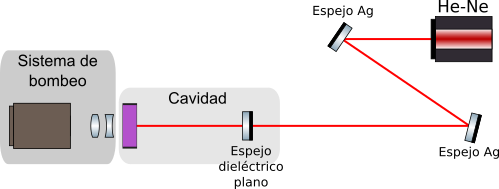
\includegraphics[scale=0.5]{Graficos/cavplana.png}
    \caption{Arreglo de la cavidad plano--paralela junto con el sistema de alineación compuesto por el láser de He--Ne y los espejos de Ag.}
    \label{cavplana}
\end{figure}

La segunda parte de la experiencia consistió en registrar distintos modos TEM. Dado que con la cavidad plano--paralela habría resultado más complicado visualizarlos, se construyó una cavidad en V (Fig. \ref{cavV1}). Teniendo en cuenta las regiones de estabilidad (Fig. \ref{estabilidad}), se tomó a = $(38.4 \pm 0.1)$cm y b = $(39.7 \pm 0.1)$cm. Previamente se habían tomado a = $(51.0 \pm 0.1)$cm y b = $(16.0 \pm 0.1)$cm, pero con esas dimensiones no se logró lasear. Para armar la cavidad en V fue necesario, en primer lugar, alinear el láser con la plano--paralela. A continuación, se colocaron un espejo dieléctrico cóncavo  (R = 50cm, HR @ 1064nm, $\phi$1") en el extremo del brazo a y un espejo dieléctrico plano en el del brazo b. Una vez alineado el sistema nuevamente, se removió el espejo que formaba la cavidad plano--paralela (el que se encontraba a 4.9cm de la barrita YAG) y se comprobó que laseara.
Para tomar una fotografía del modo TEM$_{00}$ se colocó una hoja de papel cuadriculada detrás del espejo de salida y, detrás, una cámara web. Debido a la intensidad del haz, para obtener una fotografía no saturada, fue necesario disminuir la corriente de 2.39A a 1.57A. Para evitar este problema, se colocó un espejo plano de Ag para redireccionar el haz de salida hacia una pantalla colocada a unos 5m, aproximadamente. A esa distancia fue posible observar los modos TEM y tomarles una fotografía. Para obtener los distintos modos, se modificaron minimamente las dimensiones de la cavidad con los tornillos de los posicionadores angulares. 





Por último, se generó segunda armónica. Para ello, se colocó, en el brazo b y cerca del espejo de salida, un cristal KTP (potassium titanyl phosphate). Luego, detrás del espejo de salida se ubicó un prisma para separar los haces verde e infrarrojo y se midió la variación de potencia de salida de cada haz en función de la corriente de bombeo, tal como se había hecho con el haz saliente de la cavidad plano--paralela.   







\begin{figure}[H]
    \centering
    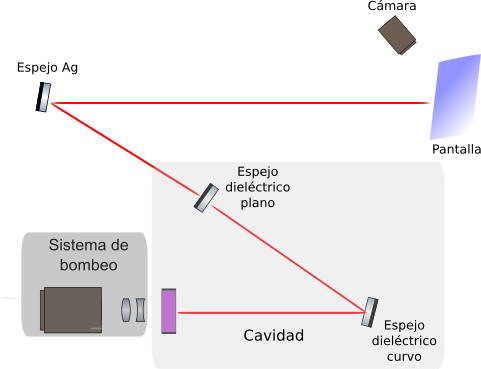
\includegraphics[scale=0.5]{Graficos/cavV1.png}
    \caption{Arreglo de la cavidad en V. Detrás del espejo de salida se colocó un espejo de Ag para redireccionar el haz hacia una pantalla ubicada a, aproximadamente, 4m.}
    \label{cavV1}
\end{figure}



%------------------------------------------------

\section*{Resultados y análisis}

Los resultados obtenidos en relación a la potencia óptica del láser fueron los esperados. En la Fig. \ref{laservscorr} se ve que la potencia óptica del láser es insignificante hasta que la corriente de bombeo alcanza 1.9A. A partir de ese umbral, la potencia aumenta de forma lineal  (R$^2$ = 0,992).
Resultaría interesante estudiar, en alguna experiencia futura, hasta qué valor de corriente se mantiene esta relación lineal.

La variación de la potencia óptica con la distancia (Fig. \ref{laservsdist}), a priori, parecen indicar que esta disminuye a medida que se aleja el sensor del láser. Sin embargo, teniendo en cuenta que una de las características de estos dispositivos es su gran colimación, se descarta esta suposición. Se cree que el porqué del comportamiento radica en la dirección del haz; es posible que este estuviera ligeramente desviado con respecto a la línea que une el láser con el sensor. Dado que el área activa del sensor es relativamente pequeña (12mm de diámetro) es posible que una pequeña desviación en el ángulo horizontal del haz produjera estos errores. Además, a pesar de haber utilizado un obturador, no se debe descartar que parte del haz del diodo de bombeo haya podido filtrarse y su potencia ser medida junto con la del láser. Esto podría explicar el comportamiento de los últimos tres puntos; de haber sido únicamente un problema de dirección del haz, los datos deberían haberse ubicado todos sobre una recta decreciente (como los primeros tres) hasta alcanzar una distancia en que la potencia fuera nula, pues el haz ya no estaría incidiendo sobre el sensor. 

\begin{figure}[H]
    \centering
    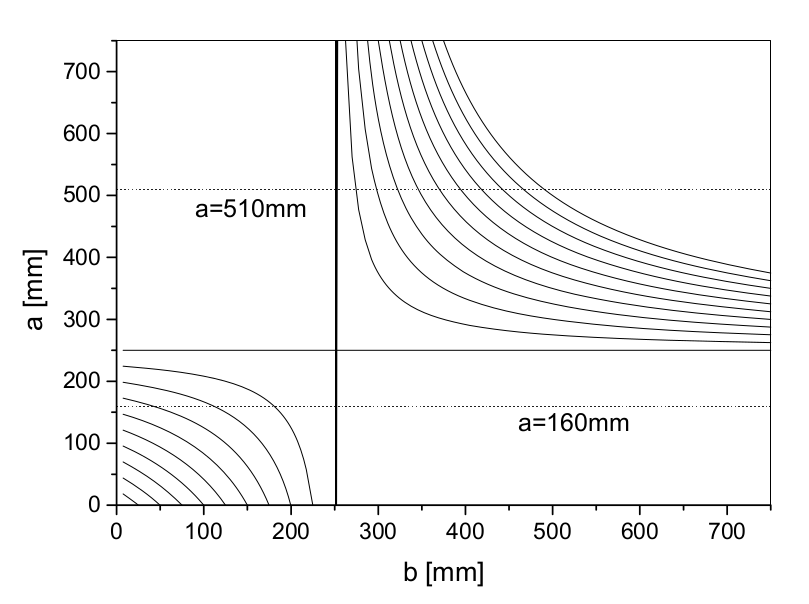
\includegraphics[scale=0.27]{Graficos/estabilidad.png}
    \caption{Regiones de estabilidad para las cavidades en V. Se muestra un ejemplo de medidas posibles para ambos brazos.}
    \label{estabilidad}
\end{figure}

Se decidió no incluir los resultados obtenidos en relación a la potencia del diodo de bombeo, dado que estas mediciones no fueron tomadas como correspondía y lo obtenido no explica el comportamiento real de la potencia. En una próxima experiencia, para medir la dependencia de la potencia óptica del diodo láser en función de la corriente y de la distancia, se deberá retirar la barra de Nd:YAG y colocar el sensor en el foco del sistema de enfoque (el haz de este láser tiene un perfil rectangular, y se utiliza un sistema de lentes que coliman el haz y lo enfocan en el Nd:YAG). Al medir a una distancia fija de $(11.5 \pm 0.1)$cm de la caja que protege el arreglo, se obtuvo un comportamiento no lineal de la potencia óptica, cuando se esperaba uno similar al de las Fig. \ref{laservscorr} y \ref{laservsdist}.

Se analizó la forma de los perfiles de intensidad de los modos TEM a partir de las fotografías obtenidas. Primeramente se corrigieron los errores introducidos por la perspectiva al tomar las fotografías utilizando un programa de manipulación de imágenes, siguiendo para este procedimiento lineamientos aceptados \cite{3}, y se aisló la región donde se observan los modos TEM propiamente dichos. Se recomienda, en caso de repetir la experiencia, contar con una cámara CCD. Con ella se podría haber medido el haz directamente y no habría sido necesaria la pantalla, con los errores que supuso a la hora de analizar los datos de forma cuantitativa.

\begin{figure}[H]
    \centering
    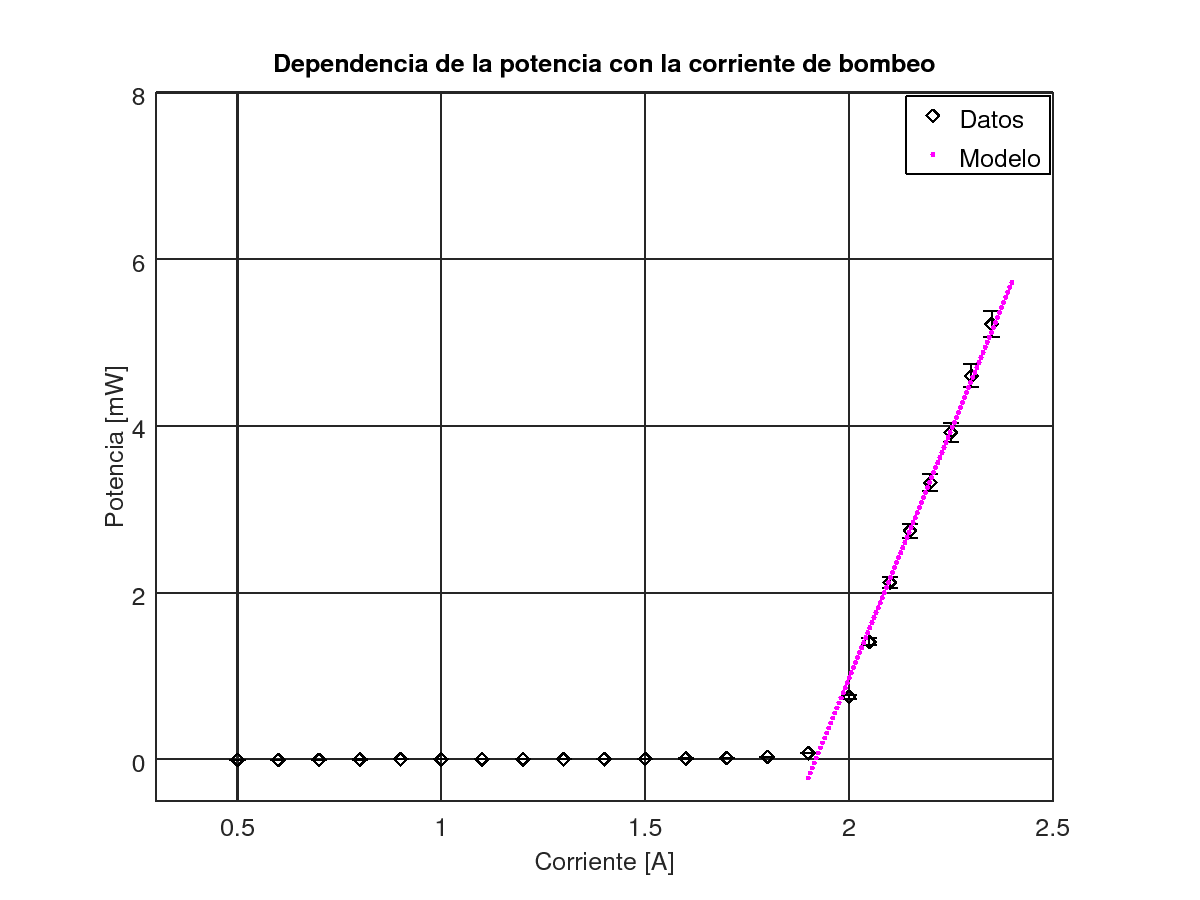
\includegraphics[scale=0.4]{Graficos/potvscor.png}
    \caption{Potencia óptica de láser en función de la corriente de bombeo. La potencia aumenta linealmente (R$^2$ = 0.992) a partir de 1.9A.}
    \label{laservscorr}
\end{figure}

\begin{figure}[H]
    \centering
    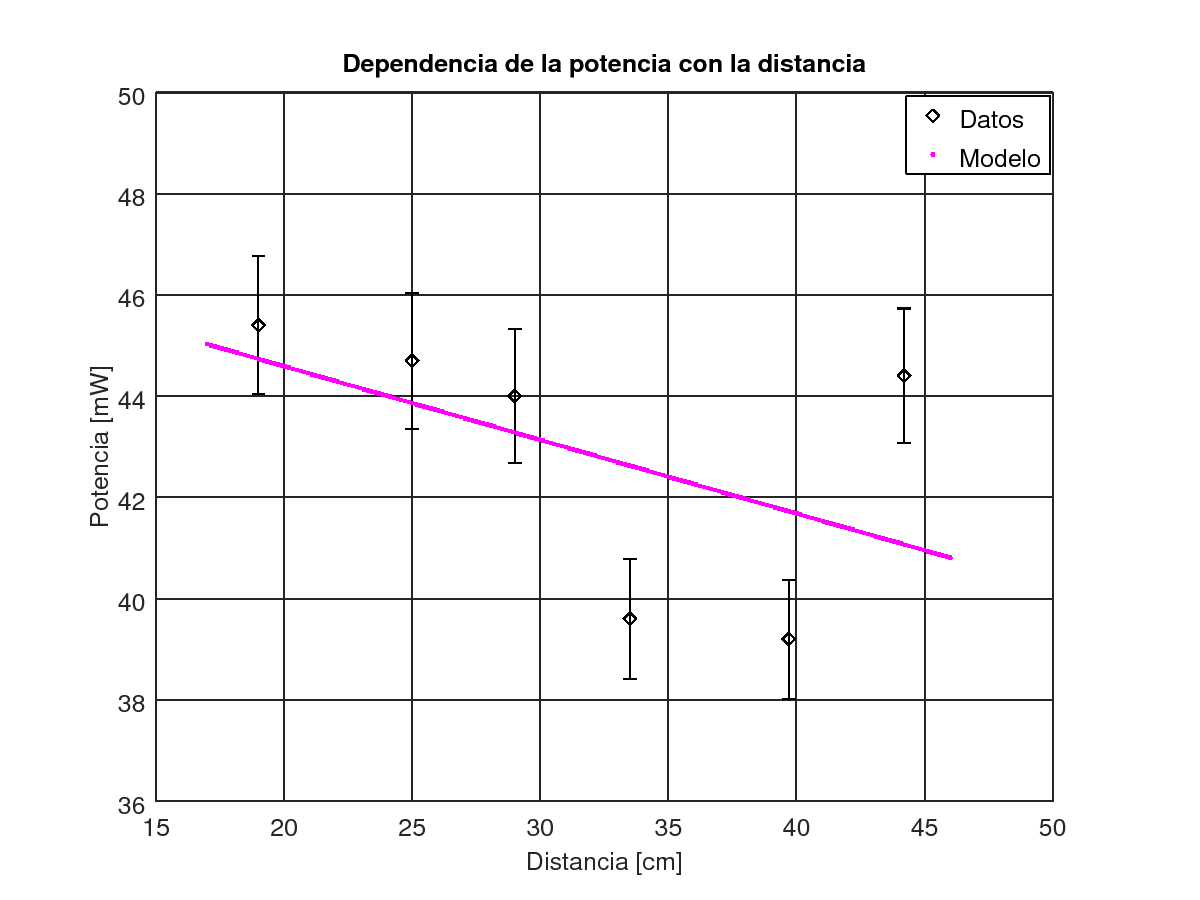
\includegraphics[scale=0.4]{Graficos/potvsdist.png}
    \caption{Potencia óptica de láser en función de la distancia para una corriente de bombeo constante de 2.39A.}
    \label{laservsdist}
\end{figure}

El procedimiento para analizar los perfiles de intensidad consistió en cargar en Python, con la librería scikit-video, cada imagen a una matriz y sumar para cada columna los valores de intensidad de cada píxel, obteniéndose luego una suma acumulada de dicho vector, el cual posteriormente se normalizó para hacer comparables entre sí los resultados de los diferentes perfiles. Esto se hizo para ambas direcciones longitudinales. 

Finalmente, se derivó la curva de intensidad para obtener, por separado, los perfiles correspondientes a cada dirección. Para estudiar si los perfiles eran los esperados según el marco teórico con que se trabajó, se modelaron las curvas de dos formas diferentes con el software Originlabs, buscando ajustar los perfiles de estas dos maneras. En primer lugar, se utilizó una función de Hermite-Gauss del orden correspondiente. Luego, a esa función se agregaron parámetros libres para compensar los errores generados por

\begin{itemize}
    \item el hecho de que el papel en donde se proyectó el haz láser no era totalmente negro,
    \item el fondo gaussiano producido por la radiación del láser de bombeo, y
    \item la variación tonal relativa debido a la reflexión del haz sobre el papel.
\end{itemize}


\begin{figure}[H]
    \centering
    
\includegraphics[scale=0.23]{Graficos/tem01.png}
    \caption{Modo TEM$_{01}$.}
    \label{fig:modo_tem01}
\end{figure}    

\begin{figure}[H]
    \centering    
    
\includegraphics[scale=0.23]{Graficos/tem11.png}
    \caption{Modo TEM$_{11}$.}
    \label{fig:modo_tem11}
\end{figure}

\begin{figure}[H]
    \centering    
    
\includegraphics[scale=0.23]{Graficos/tem02.png}
    \caption{Modo TEM$_{02}$.}
    \label{fig:modo_tem02}
\end{figure}


\begin{figure}[H]
    \centering    
    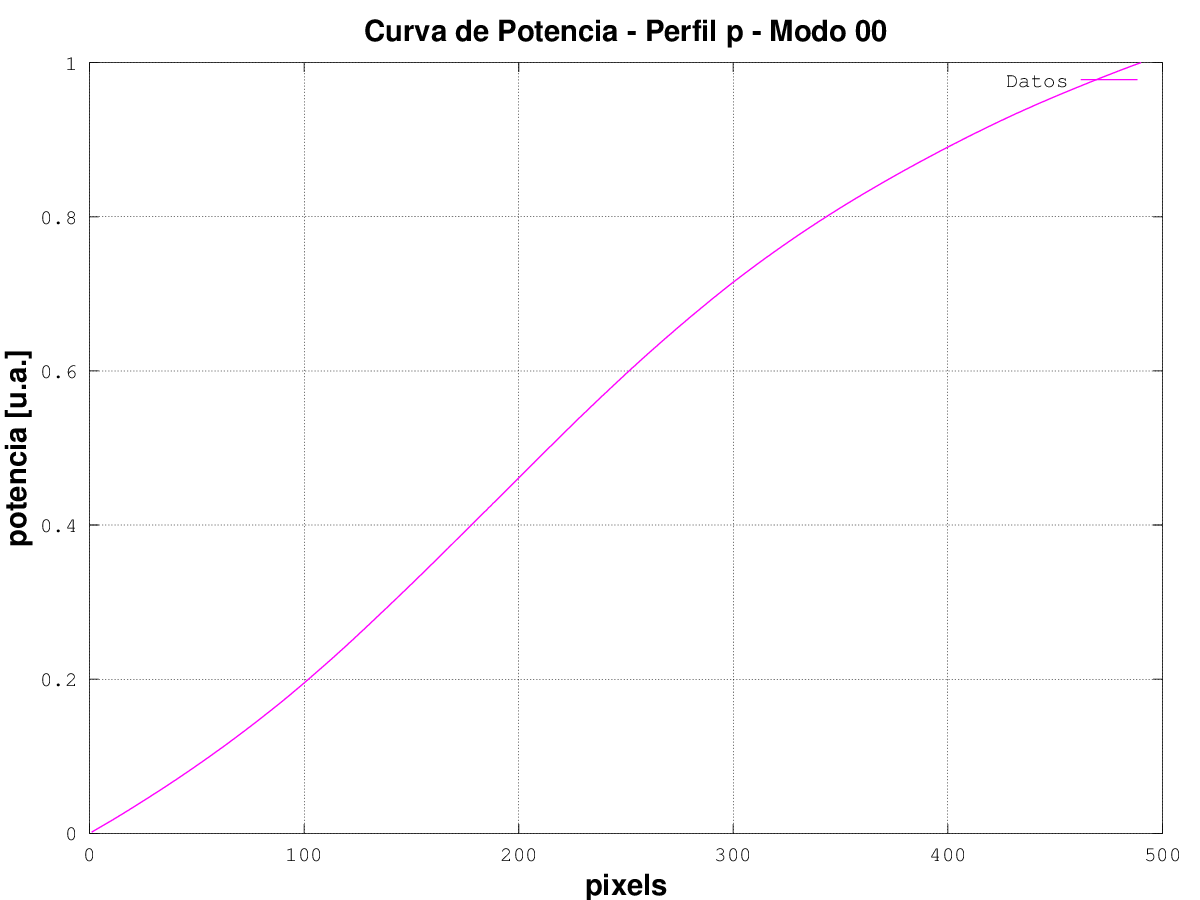
\includegraphics[scale=0.35]{Graficos/plt_pot_tem00.png}
    \caption{Curva de Potencia Normalizada para el perfil p del modo TEM$_{00}$.}
    \label{fig:pot_modo_tem00}
\end{figure}

\begin{figure}[H]
    \centering    
    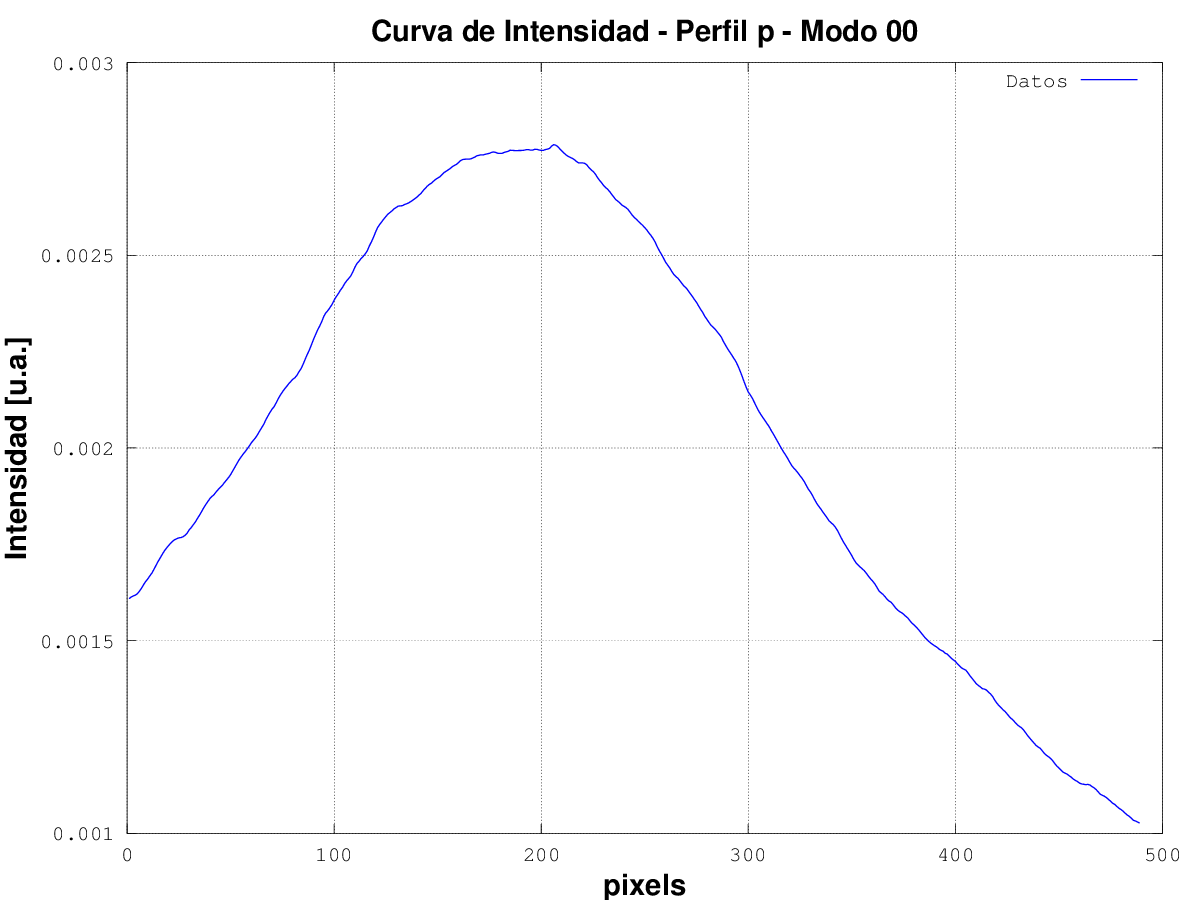
\includegraphics[scale=0.35]{Graficos/plt_int_tem00_perfil_p.png}
    \caption{Curva de Intensidad Normalizada para el perfil p del modo TEM$_{00}$.}
    \label{fig:int_modo_tem00}
\end{figure}



Cuando se intentó ajustar las curvas obtenidas a partir del análisis de las imágenes sin compensar estos errores, no se obtuvieron los resultados esperados. Sin embargo, para órdenes bajos de los modos TEM, el ajuste que contempló los errores metodológicos logró converger a una función que se corroboró con las curvas obtenidas a partir de las imágenes. Aun así, este modelo falló para órdenes mayores a 3 debido a que los máximos de intensidad estaban demasiado cerca, lo que impedía que fueran discernidos apropiadamente.

Una vez generada segunda armónica y separados los haces verde e infrarrojo, se midió la potencia de cada uno y los resultados son los que se muestran en las Fig. \ref{potverde} y \ref{potrojo}. La potencia del haz infrarrojo mostró un comportamiento lineal (R$^2$ = 0.994), tal como se esperaba. En este caso, el umbral de corriente fue más bajo que para el caso de la Fig. \ref{laservscorr}; concretamente, se pasó de un umbral de 1.9A a uno de 1.46A. Si bien en ambos casos se estaba trabajando con cavidades estables, la plano--paralela es menos estable que la cavidad en V (por eso se utilizó esta configuración para observar los modos TEM), y por eso era necesaria más corriente para que el láser emitiera haz. Por cuestiones de tiempo no se registraron datos a corrientes menores de 1.46A, aunque sí se verificó, realizando un barrido de corriente, que la potencia para valores inferiores a 1.46A era nula. 

Con respecto a lo obtenido para la potencia del haz verde, no se tiene una explicación satisfactoria. Hay un punto (potencia a 1.1A) que presenta un salto. Dado que es un hecho aislado, se atribuye a un salto de tipo eléctrico y no relacionado con el comportamiento de la potencia en sí. Resultados de experiencias previas indicaban que este comportamiento debería haber sido cuadrático a partir de un cierto umbral de corriente. Se tomó la región donde la potencia del haz infrarrojo era lineal y se modelaron los datos del haz verde con una función lineal y con una cuadrática. A simple vista, ambos ajustes parecen adecuados, aunque la parábola explica algo mejor los datos. Para compararlos, en este caso se tomaron los residuos: 2.7$\times$10$^{-3}$ y  7.92$\times$10$^{-4}$ respectivamente. Entonces, se podría decir que el modelo cuadrático es mejor. Sin embargo, teniendo en cuenta los órdenes de magnitud de los residuos, una recta también podría explicar el comportamiento, por lo menos a primer orden. Por tanto, no se puede afirmar que haya un comportamiento cuadrático predominante. Una hipótesis es que puede haber cambiado el modo del láser con valores distintos de corrientes, aunque no se está en grado de corroborarlo. Se descarta una influencia del cristal KTP o del prisma, por ser materiales con alto umbral de daño y estabilidad térmica; asimismo, se tuvo la precaución de enfocar el sensor sobre cada haz por separado, centrándolo en el área activa. En estas condiciones, es necesario repetir las mediciones para poder explicar el comportamiento de la potencia del haz verde.

\begin{figure}[H]
    \centering    
    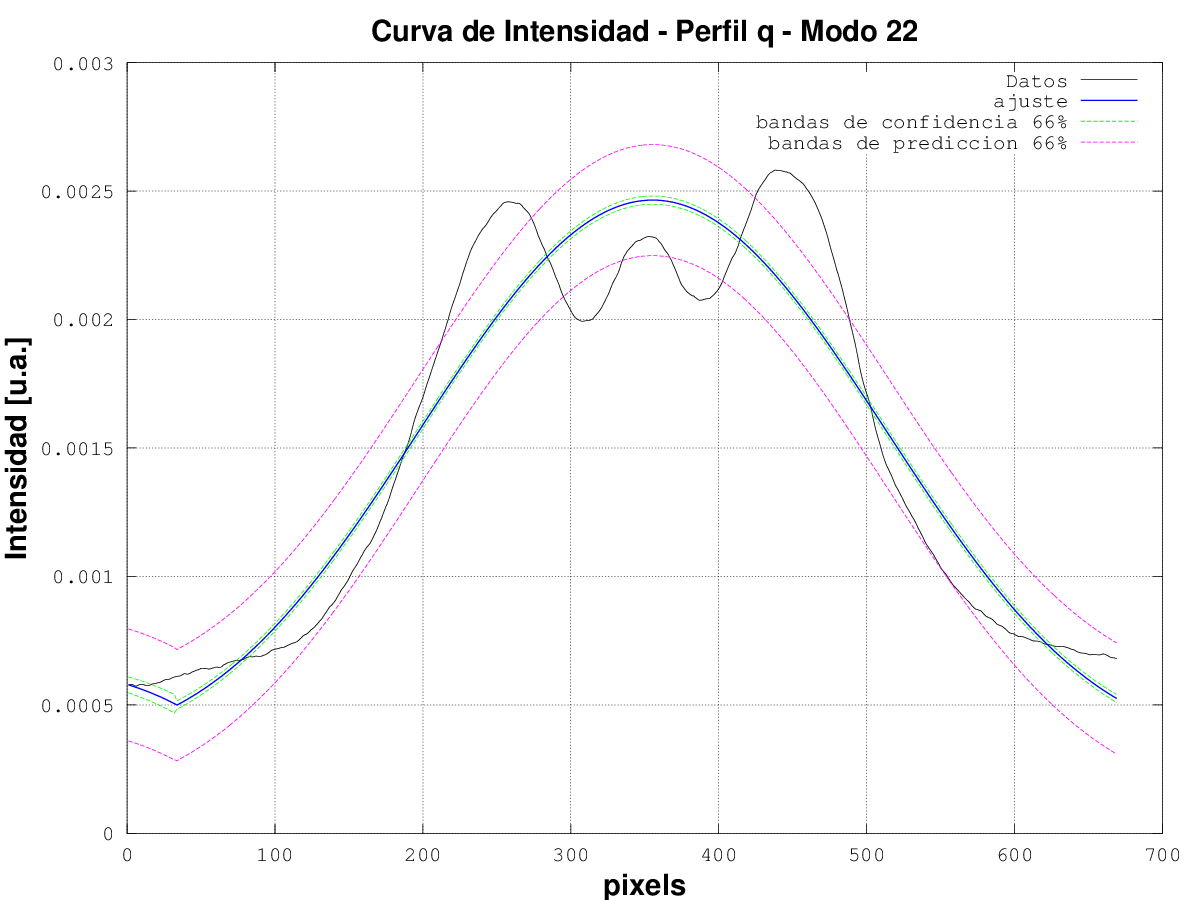
\includegraphics[scale=0.35]{Graficos/plt_ajuste_tem22_perfil_q.png}
    \caption{Ajuste sin compensar errores para el perfil q del modo TEM$_{22}$.}
    \label{fig:ajuste_malo_modo_tem22}
\end{figure}
\begin{figure}[H]
    \centering    
    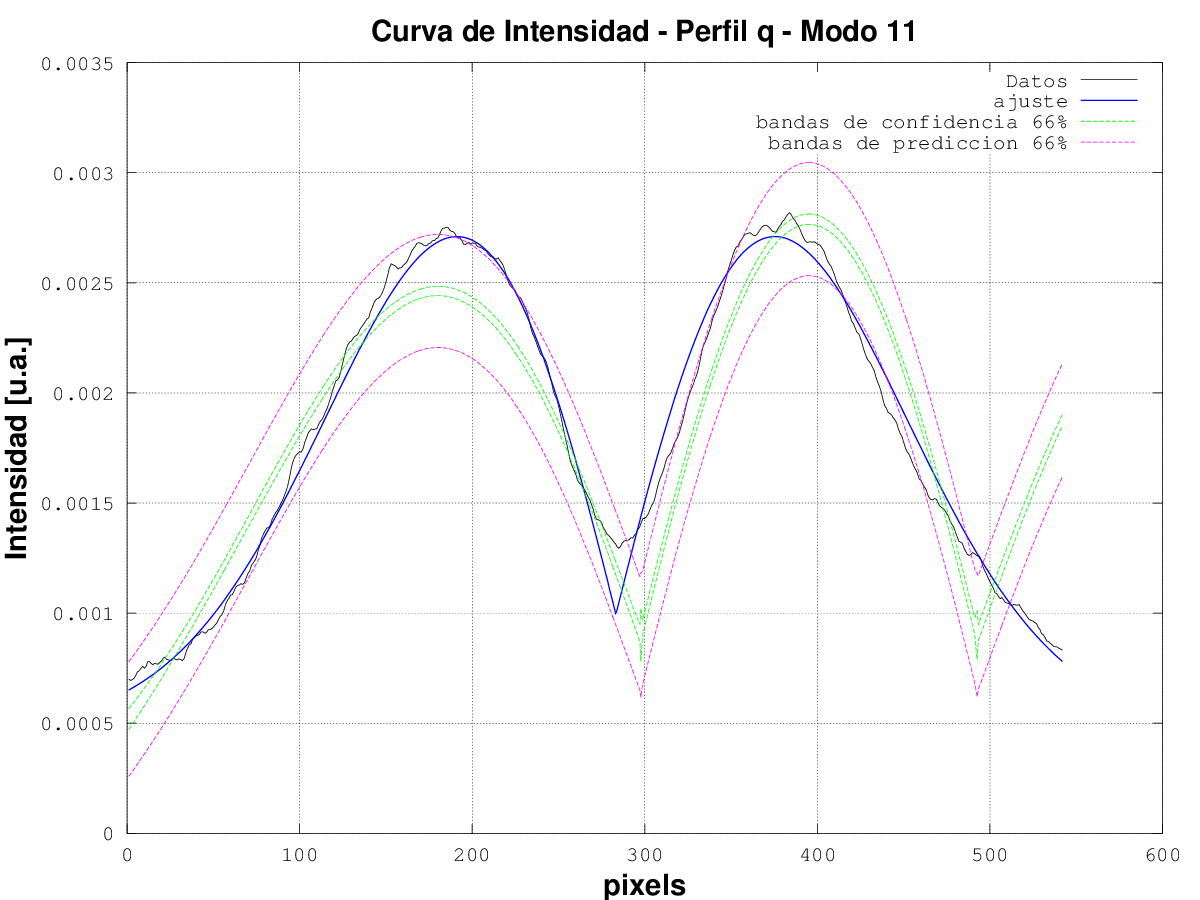
\includegraphics[scale=0.35]{Graficos/plt_ajuste_tem11_perfil_q.png}
    \caption{Ajuste compensando errores para el perfil q del modo TEM$_{11}$.}
    \label{fig:ajuste_bueno_modo_tem11}
\end{figure}
\begin{figure}[H]
    \centering    
    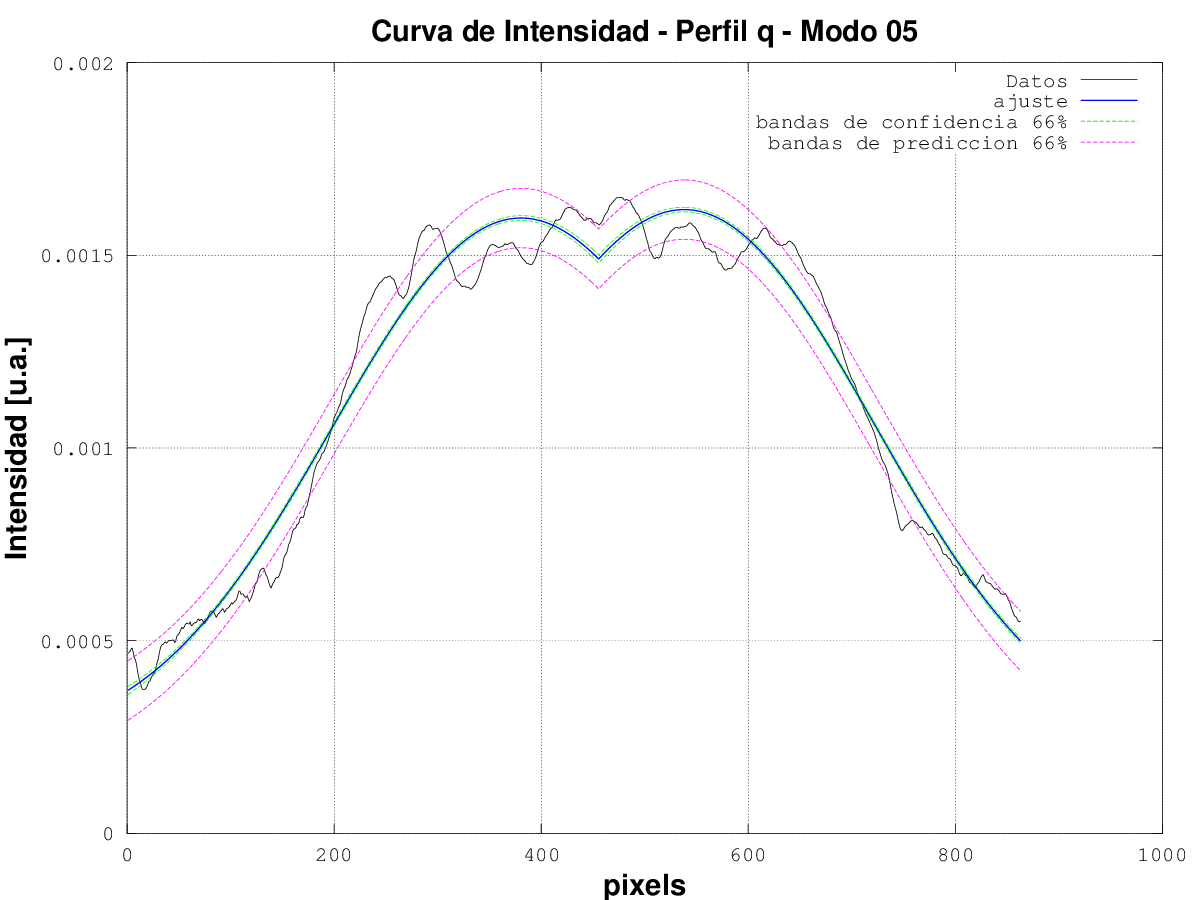
\includegraphics[scale=0.35]{Graficos/plt_ajuste_tem05_perfil_q.png}
    \caption{Ajuste compensando errores para el perfil q del modo TEM$_{05}$.}
    \label{fig:ajuste_malo_modo_tem05}
\end{figure}


\section*{Conclusiones}
% \addcontentsline{toc}{section}{Conclusiones} % Adds this section to the table of contents
En este trabajo se presentaron los resultados de las experiencias realizadas. En primer lugar se construyó una una cavidad plano--paralela y se midió la potencia óptica de salida tanto del láser como del diodo de bombeo en función de la corriente y de la distancia. Para el caso del láser, la dependencia con la corriente mostró el perfil lineal esperado. Se observó que la potencia presentaba una tendencia a disminuir con la distancia, pero se concluyó que esto ocurría por una desviación del sensor con respecto al haz y no por una divergencia del mismo. Los resultados obtenidos para la potencia del diodo de bombeo se omitieron por no haber realizado las mediciones como correspondía. 


\begin{figure}[H]
    \centering
    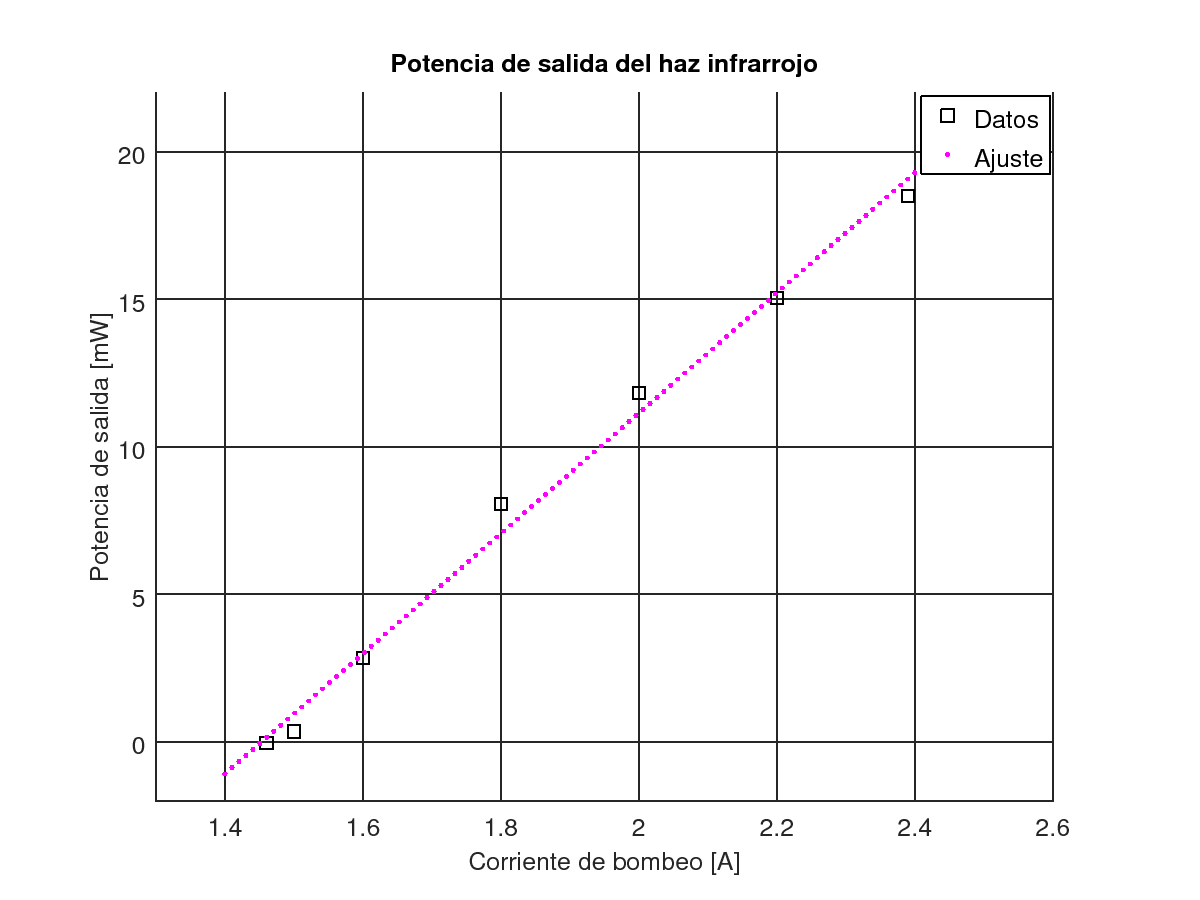
\includegraphics[scale=0.4]{Graficos/pot_infrarrojo.png}
    \caption{Potencia de haz infrarrojo en función de la corriente de bombeo. La potencia aumenta linealmente (R$^2$ = 0.994) a partir de 1.46A.}
    \label{potrojo}
\end{figure}
\begin{figure}[H]
    \centering
    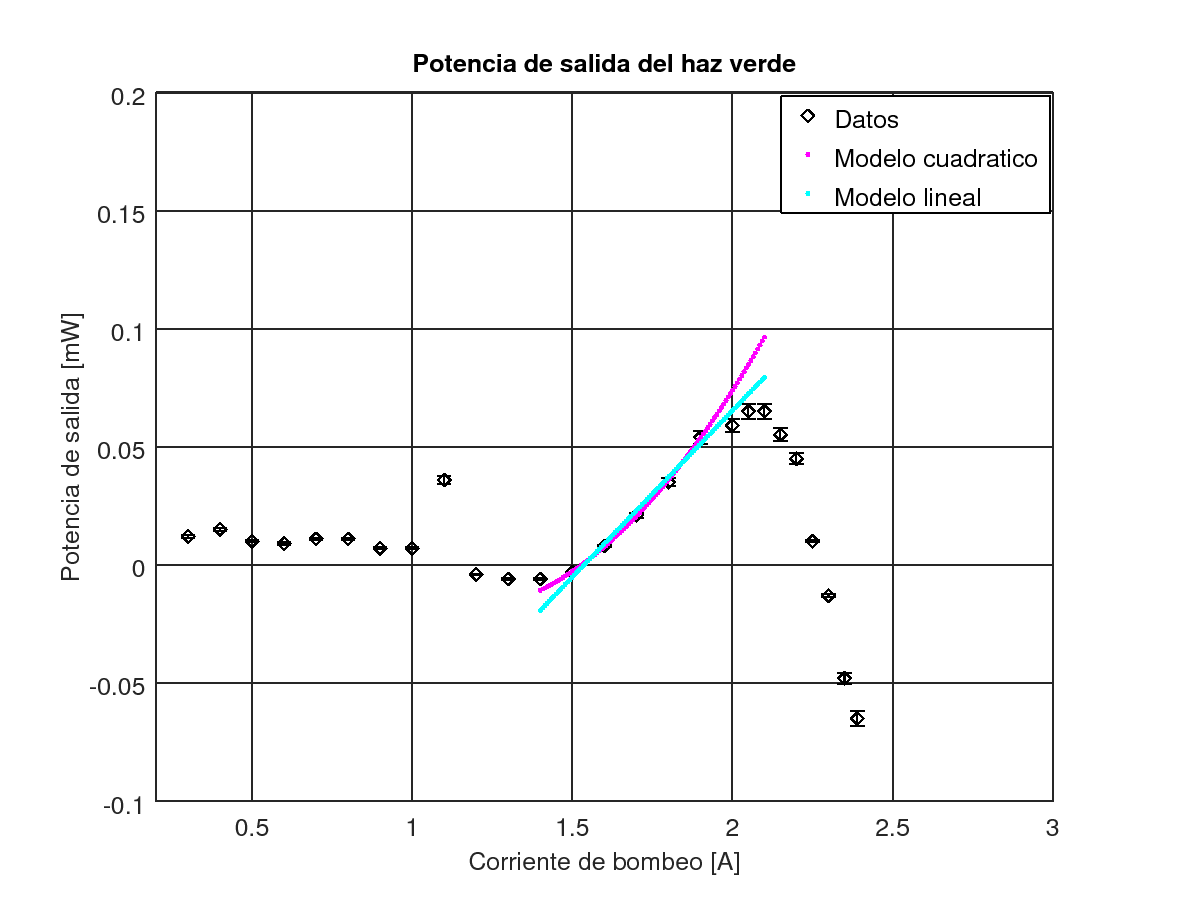
\includegraphics[scale=0.4]{Graficos/pot_verde1.png}
    \caption{Potencia del haz verde en función de la corriente de bombeo. Se observa un comportamiento anómalo de los datos.}
    \label{potverde}
\end{figure}




Luego se construyó una cavidad en V y se pudieron observar de manera cualitativa que diferentes modos TEM obtenidos al variar la longitud de la cavidad en V se correspondendían con lo predicho por la teoría. Si bien en el análisis cuantitativo se tuvieron dificultades al identificarse la correlación con la teoría de manera directa debido a los errores introducidos por el procedimiento experimental, sí se comprobó dicha correlación al tenerse en cuenta  estos errores. Una de las mayores dificultades al obtener las imágenes de los modos es que al momento de la medición no había a disposición cámaras CCD en funcionamiento con las cuales obtener directamente información de los perfiles de intensidad. Una vez registrados los modos TEM, se generó segunda armónica con un cristal KTP y se dividió el haz con un prisma. Se registró la dependencia de la potencia de ambos haces con la corriente, obteniendo los resultados predichos para el caso del infrarrojo, pero no para el verde. No se cuenta en este momento con una explicación de este comportamiento, aunque una hipótesis es que podría haber cambiado el modo. Es necesario repetir la experiencia para estar en grado de dar una explicación. Una medición que se propone para quien realice la experiencia en el futuro sería ver si se mantiene la linealidad de la potencia (para el haz infrarrojo) para valores mayores de corriente que los utilizados.





%----------------------------------------------------------------------------------------
%	BIBLIOGRAPHY
%----------------------------------------------------------------------------------------


\begin{thebibliography}{100}
\bibitem{1}{Apuntes de la materia, \url{http://users.df.uba.ar/bragas/Labo5_1er2011/laser2k.pdf}}
\bibitem{2}{Robert W. Boyd, \textit{Nonlinear Optics}, 3ra edición, Academic Press, Inc, 2008.}
\bibitem{3}{Douglas W. Cromey, \textit{Avoiding Twisted Pixels: Ethical Guidelines for the Appropriate Use and Manipulation of Scientific Digital Images}, Sci Eng Ethics. Dec (2010) , Volume 16(4), Pages 639–667. }
\end{thebibliography}
%----------------------------------------------------------------------------------------
\end{multicols}
\end{document}
